\chapter{Classical numerical results and Benchmarks} % Main chapter title

\label{Chapter3} % Change X to a consecutive number; for referencing this chapter elsewhere, use \ref{ChapterX}

In last section we saw that the American put was an example of an option that required numerical procedures to be priced fair. The American put is far from the only example of a derivative without a closed-form solution. We will look at two classical valuation algorithms for pricing American options in computational finance the Cox-Ross-Rubinstein (CRR) binomial model \parencite{CRR} and the Least Square Monte Carlo (LSM \parencite{LSM}). The binomial model is an example of a strategy to approximate the option by discretization of the underlying risky asset(s) and the LSM is a method to simulate the underlying risky asset(s). Another popular choice is to solve the free boundary problem with finite difference methods, but we chose to focus on the two other numerical procedures. The chapter will also investigate valuing exotic multivariate contingent claims. We extend the binomial pricing model (\parencite{NEK,BEG}) and LSM to multivariate contingent claims and provide some closed form solutions for exotic European options (\parencite{Johnson87, Ouwehand2006}). We wrap up the chapter with numerical findings. Therefore the chapter have two purposes to gain insight into valuation for exotic options and provide some benchmarks for the Neural Network in the coming chapters.

%----------------------------------------------------------------------------------------
%	SECTION 1
%----------------------------------------------------------------------------------------
\section{Cox Ross Rubenstein Model}\label{CRR}
The classical binomial model pricing formula or the CRR model presented in this section is inspired by \parencite{CRR,Hull,finKont}. The model will be used for pricing an American put option with 1 underlying stock and to build the foundation for pricing bivariate contingent claims with the binomial model \parencite{BEG}. The CRR model provides an intuitive and easy implementable model for valuing American and European options. The binomial model comes handy, when no analytical model exists e.g. for an American put option. The binomial model also has its limitations, because for computational reasons it is not suited for valuing path dependent options or options with several underlying factors. The key difference on the binomial model and the simulation approach is that the binomial model discretize the underlying stochastic process(es) in time. \\

Assume the same market and Black-Scholes assumptions as in chapter 2, but the underlying stochastic process will be assumed to follow a multiplicative binomial process over discrete periods. We work with the financial market $(\Omega, \mathcal{F}, \mathbb{F}, P, S_0, S_1)$, where the filtration is generated by $\mathbb{F}= \sigma(\mathcal{F}_{t_n})_{n=0,1,\ldots, N}$ and the sigma algebra is chosen to be $\mathcal{F}=\mathcal{F}_{t_{N}}$. It is well known from discrete arbitrage theory, that the binomial market model with two assets, where $u>1+r>d>0$ is a complete and arbitrage free model. The u,d and r describes the evolution of the discrete stochastic process for the stock and the free interest rate on the bank account. 
\begin{align*}
S_{0}(t_n)=S_{0}(t_{n-1}) \cdot \exp(\Delta t \cdot r) \quad where \ S_{0}(0)=1 \ and \ n=0, \ldots, N\\
S_{1}(t_n)=S_{1}(0)\prod_{j=1}^{n} Y_{j} \quad where \ Y_1,Y_2, \ldots, Y_N \ are \ i.i.d., \ S_1(0)>0
\end{align*}
Note that the interest rate is continuously compounded for computational convenience and the equidistant time step is $\Delta t=T/N$ (section \ref{DiscreteValueFramework} for notation). We assume that \[ Y_i = \begin{cases} 
      u & with \ probability \ p \\
      d & with \ probability \ (1-p)
   \end{cases}
\]

Below a illustration of a discrete multiplicative binomial process with two time steps, where the lattice recombines.

\begin{figure}[H]
\centering
% Define styles for bags and leafs
\tikzstyle{bag} = [text width=2em, text centered]
\tikzstyle{end} = []
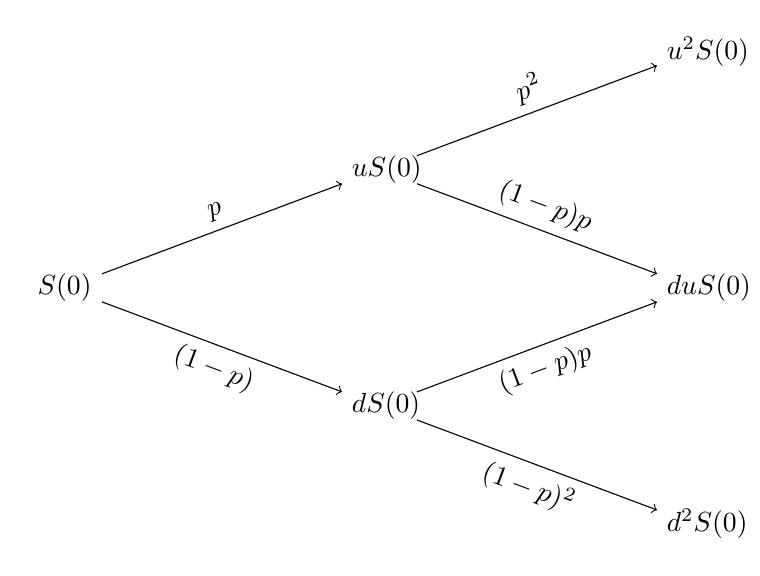
\begin{tikzpicture}[sloped]
   \node (a) at ( 0,0) [bag] {$S(0)$};
   \node (b) at ( 4,-1.5) [bag] {$d S(0)$};
   \node (c) at ( 4,1.5) [bag] {$u S(0)$};
   \node (d) at ( 8,-3) [bag] {$d^2 S(0)$};
   \node (e) at ( 8,0) [bag] {$d u S(0)$};
   \node (f) at ( 8,3) [bag] {$u^2 S(0)$};
   \draw [->] (a) to node [below] {$(1-p)$} (b);
   \draw [->] (a) to node [above] {$p$} (c);
   \draw [->] (c) to node [above] {$p^2$} (f);
   \draw [->] (c) to node [above] {$(1-p)p$} (e);
   \draw [->] (b) to node [below] {$(1-p)p$} (e);
   \draw [->] (b) to node [below] {$(1-p)^2$} (d);
\end{tikzpicture}
\decoRule
\caption[Two Dimensional Binomial Lattice]{Price dynamics of binomial model with one underlying risky asset with N=2, $S(0)$ is spot value, p objective probability measure, u and d is realizations of the stochastic variable $Y_i$}
\label{fig:twoDimLattice}
\end{figure}

By constructing the discrete process for the stock it is easy to find the equivalent martingale measure. 
\begin{definition}\label{findQ}
Assume there exists a risk free asset. A probability measure $Q$ is called a martingale measure if the following condition holds 
\begin{align}
s= \exp(- r \Delta t) \cdot E^Q[S(t+\Delta t)|S(t)=s] 
\end{align}
Where $\Delta t$ is a single time-step (p. 18 \parencite{Bjork19}).
\end{definition}
By using definition \ref{findQ} we find the risk neutral measure to be:
$$q=\frac{e^{r \Delta t}-d}{u-d}$$
The martingale measure q is unique in the binomial model, because the model is complete. By above assumption about $u>1+r>d>0$ the binomial model with the market ($S_0(t_n), S_1(t_n)$) is a arbitrage free and complete model, hence to the general pricing formula is given by the risk neutral valuation formula.
\begin{theorem}\label{RNVF-Discrete}
\textbf{Risk-neutral valuation formula (RVNF) in discrete time for T-claim}
The arbitrage free price at t=0 of a T-claim $X$ is given by
\begin{align}
\Pi(0;X)&= \exp(- r \Delta t \cdot N) \cdot E^Q[X]\\
&=\exp(- r \Delta t \cdot N) \cdot \sum_{n=0}^{N} \binom{N}{n} q^n (1-q)^{N-n} \Phi(su^n d^{N-n})
\end{align}
here $Q$ denotes the martingale measure, $\Pi(0;X)$ is the price of X to time 0 and $\Delta t$ is a single time step (p. 25 \parencite{Bjork19}).
\end{theorem}

By above formula the binomial model gives a simple mathematical framework for pricing European options, but the model can easily be extended to American options. American put options for the binomial will be solve with the dynamic programming approach, because the binomial model gives a recursive formula where the one-step transition probabilities are the same in each node.
\begin{equation}\label{BellmanEq2}
\begin{split}
\begin{cases}
          P(t_i) = max\{ (K-S(t_i))^+, \exp(-r\cdot \Delta t) E^Q[P(t_{i+1})|S(t_i)])\} \quad for \ i={0,\ldots,N-1} \\
          P(t_N) = (K-S(t_N))^+ 
\end{cases}
\end{split}
\end{equation}
The idea is to at each decision point either exercise to gain the intrinsic value or hold the option alive for another period. The value of keeping the option alive is called the expected continuation value and it is given by the risk neutral valuation formula. The dynamic choice to exercise or to keep the option alive gives a exercise barrier $b$ (see section \ref{AmericanPut}).\\

So to value an American put option, we lay out all the possible path of the stock based on $S_1(0),\sigma$ and $T$. These paths construct the tree, then for valuation we work backwards in the tree starting at maturity. Figure \ref{fig:BinomialTree} is an example of a constructed tree, where the value of the option is also included by color. The decision to exercise is marked with a triangle where the decision points where is optimal to keep the option alive is marked with circles. \\

\begin{figure}[th]
\centering
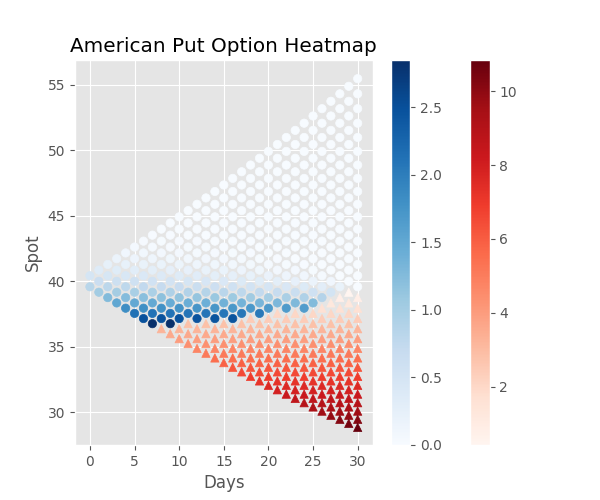
\includegraphics{Figures/BinomialTree.png}
\decoRule
\caption[Binomial Tree]{A valuation tree of an American put option price based on the binomial model, where the color indicate the value and the dots are marking the continuation nodes. The parameters are S(0)=40, N=30, $\Delta t =$ 1 day, K=40 and u=1.0106}
\label{fig:BinomialTree}
\end{figure}

To construct the tree we need to specify the number of equidistant time-steps $\Delta t$ ($\Delta t = \frac{T}{N} \ where \ N=No. \ of  \ steps$) for the tree, where for each step we add another possible value for the stock. We only add 1 more possibility for each time-step because the tree recombines \footnote{$(1+n)$ possible stock values after n steps}. The d and u is chosen such that they match volatility.
$$u= \exp(\sigma \sqrt{\Delta t}) \quad d= \exp(-\sigma \sqrt{\Delta t})$$
For valuing an American put option, we value the exercise value at maturity (time T) for all possible outcomes for the price process at maturity. Then we use backward induction/dynamic programming where we compare the intrinsic value with the expected continuation value (equation \eqref{BellmanEq2}), where we choose the maximum of these two. The comparison will be applied for every node in each decision point $(t_{n})_{n=0,1,\ldots,N-1}$ and all the way back in time to the initialization date. By this procedure we get present value of the American option. One design decision is to choose number of time-steps considering a trade-off between computational efficiency and accuracy. Figure \ref{fig:binConv} illustrates that around 40 steps the option value stabilizes for an option with 1 year to maturity. The precision for the algorithm increases with the number of steps and the option value stabilizes for increasing number of steps (see Figure \ref{fig:binConv}).\\

\begin{figure}[th]
\centering
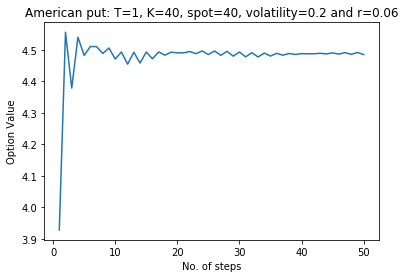
\includegraphics{Figures/binConv.png}
\decoRule
\caption[Convergence Of Binomial Model]{Price for a American put option based on the binomial model, where the independent variable is the number of time-steps. Vol. is an abbreviation for volatility.}
\label{fig:binConv}
\end{figure}

We have seen the central concepts arbitrage and completeness from continuous time in action for the discrete time setup. The paper \parencite{CRR} which introduced the binomial model to option pricing came after the Black-Scholes model described in section \ref{Chapter2} \parencite{B-S-Paper}. The main reason for developing a model in discrete time is that the discrete time approach gives a simplified model in terms of the mathematics and highlights the essential concepts in arbitrage theory. You can argue that the simpler mathematics in this model makes the binomial model more instructive and clear. Besides being easier to understand for non-mathematician it works nicely with other options than the European options like American options. Even though we assume the stock price moves at discrete jumps instead of the classical Black-Scholes continuous time model, it can actually be shown that the CRR binomial model will converge to the continuous time model. Hence the binomial pricing model will be equivalent with the continuous time analytical pricing model derived by Fischer Black and Myron Scholes in the limit for European options for sufficient small time steps. \\

Note for computational resources the path-independence payoff for the American put makes the tree recombining is important, so there is only N+1 terminal nodes at maturity. If the derivative was path-dependent e.g. an Asian option, then we have a non-recombining tree and $2^{N}$ terminal nodes where needed. This is a computational inefficient, which explains that the binomial model should not be used for path-depending derivatives. The problem with a derivative with several underlying e.g. a basket option is also the increasing number of nodes, because now you have $2^d$ possible one-step transitions. We will show below that the intuitive CRR binomial model can be extended to higher dimensions, but the model suffers from the curse of dimensionality.

\newpage
%----------------------------------------------------------------------------------------
%	SECTION 2
%----------------------------------------------------------------------------------------
\section{Lattice Approach For Multivariate Contingent Claims}
We follow the approach in \parencite{BEG} (BEG method), because it is the natural extension of the Cox Ross Rubinstein model (section \ref{CRR}) for multivariate contingent claims. The idea as in the one dimensionel case is to approximate the system of underlying processes (assumed to be GBMs) with a discrete multivariate binomial lattice. The advantage is that for exotic options like the rainbow options the valuation of European put options is readily extended to the American put options and has high accuracy. The \parencite{BEG} has its limitation in terms of number of underlying assets and for path dependent options (see section \ref{CRR}), but it is very intuitive and extends easily to American options. The problem with increasing the number of underlying assets is that the number of one-step transition at each node is $2^d$ and the total number of terminal nodes after N steps is $(N+1)^d$ for path-independent derivatives, which means for high dimensional problems the computational resources become an issue with this discrete approximation approach. This makes the BEG method undesirable for higher dimensions than three so we will focus on the two dimensional case. Another problem with three or more underlying assets are that some one-step transition probabilities can turnout negative with the BEG method, which makes the model nonsense in those cases. \\

The model we want to approximate is the bivariate lognormal distribution, because we assume the Black-Scholes model to describe the evolution of the two risky assets (section \ref{MultiDimModel}). We restrict ourselves to the assumptions \ref{BS-Assumption} given in the classical \parencite{B-S-Paper}, hence for risk neutral pricing the SDE for the risky assets are:
$$dS_i(t)=S_i(t)r(t)dt+S_i(t)\sigma_i(t)dW^Q(t) \quad for \ i=1,2,\ldots,d$$
We divide the time from inception to maturity (length T) into N equidistant intervals with length $\Delta t$, because we want the jump distribution to approximate the continuous time multivariate lognormal distribution. Each time interval has a jump size defined in terms of the volatility and the length of the interval:
$$u_i=\exp(\sigma_i \sqrt{\Delta t}) \quad and \quad u_i \cdot d_i = 1 \quad for \ i=1,2,\ldots,d $$
The $u_i$ and $d_i$ are the multiplication factor for the i'th stock, where the former is a jump up and the latter is a jump down for the stock. What is the probability that the stock jumps up or down? The probabilities are chosen such that the characteristics functions are equal for small time steps $\Delta t$ (see p. 245-246 in \parencite{BEG} for details). The probabilities for the model with two underlying risky assets:
\begin{equation}
\begin{split}
p_1=p_{uu}=\dfrac{1}{4}\bigg( 1+\rho + \sqrt{\Delta t}(\dfrac{\mu_1}{\sigma_1} + \dfrac{\mu_2}{\sigma_2}) \bigg)\\
p_2=p_{ud}=\dfrac{1}{4}\bigg( 1-\rho + \sqrt{\Delta t}(\dfrac{\mu_1}{\sigma_1} - \dfrac{\mu_2}{\sigma_2}) \bigg)\\
p_3=p_{du}=\dfrac{1}{4}\bigg( 1-\rho + \sqrt{\Delta t}(-\dfrac{\mu_1}{\sigma_1} + \dfrac{\mu_2}{\sigma_2}) \bigg)\\
p_4=p_{dd}=\dfrac{1}{4}\bigg( 1+\rho + \sqrt{\Delta t}(-\dfrac{\mu_1}{\sigma_1} - \dfrac{\mu_2}{\sigma_2}) \bigg)
\end{split}
\end{equation} 
The correlation $\rho$ between the two assets are assumed to be constant and $\mu_i=r-\frac{1}{2}\sigma_i^2$. We have illustrated below a two-dimensional lattice, where we see that the number of nodes at maturity is $(1+N)^d$. 

\begin{figure}[th]
\centering
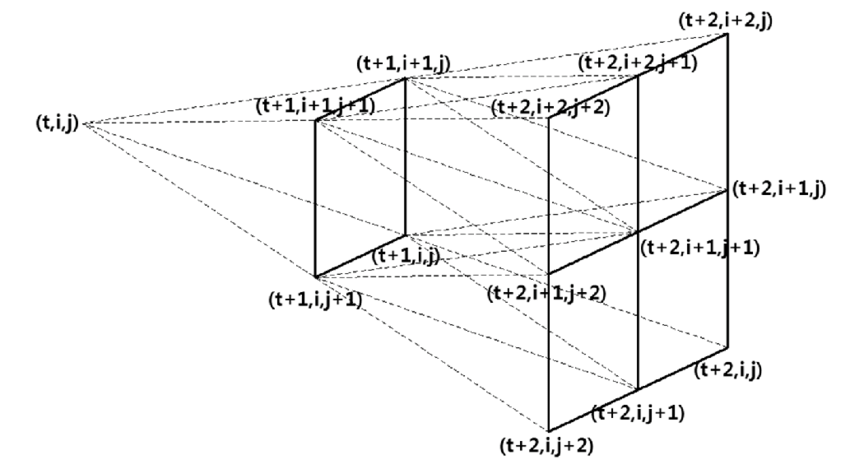
\includegraphics[width=\textwidth]{Figures/Three-dimensional-binomial-lattice.png}
\decoRule
\caption[Three Dimensional Binomial Lattice]{Evolution of binomial model with two underlying risky asset, where t is time, i is number of up movement for $S_1$ and j is number of up movement for $S_2$.}
\label{fig:threeDimLattice}
\end{figure}

After the construction of the evolution of the underlying assets, we can like in the one dimensional CRR model recursively working backward in the multidimensional binomial lattice. For the European option the recursive formula is:
$$V_{i_1,\ldots, i_d}(t)=\exp(-r\Delta t) \bigg(p_1 V_{i_1+1,\ldots, i_d +1}(t+1) + \cdots + p_{2^d} V_{i_1,\ldots, i_d}(t+1) \bigg)$$
For the American option we approximate it with the Bermudan option with N-1 decision points, hence we have the possibility of exercising between inception and maturity of the contract at the decision points hence:
$$V_{i_1,\ldots, i_d}(t)=\max\{\Phi(t,\bm{S}(t)), \exp(-r\Delta t) \bigg(p_1 V_{i_1+1,\ldots, i_d +1}(t+1) + \cdots + p_{2^d} V_{i_1,\ldots, i_d}(t+1) \bigg)\}$$
With the recursive formulas we can valuate multivariate contingent claims for a variety of exotics including the American put option with several underlying risky assets. The increasing dimensions also increase the number of one-step transition probabilities, hence the \parencite{NEK} approach (NEK) tries with setting all the probabilities equal to 0.5 and than determine the jump sizes. The NEK approach overcome the issue with negative probabilities for higher dimensions and following \parencite{NEK} the algorithm seems also to have faster convergence. The NEK and BEG approaches are both good in terms of both accuracy and computational speed for low dimensional option problems, but both still suffers from the curse of dimensionality. The simulations methods on the other hand has somewhat an advantage for higher dimensions. We choose to present the BEG approach, because it is a natural extension of the already presented CRR model, which we already build intuition upon. The key for the BEG approach is that we approximate a multivariate lognormal distribution with a discrete distribution. 

\newpage

\section{Least Square Monte Carlo Method}\label{LSM}
From above the binomial model is not suitable for path-dependent contingent claims like an Asian option and high dimensional multivariate contingent claims. Simulation methods overcome somewhat this issue. The first Monte Carlo methods was to use pure simulation techniques, these methods overcome the issue of path-dependent option, but they still suffered the curse of dimensionality. To solve the dimensionality problem the LSM was born, where the idea is combine simulation with regression. \\

A pure simulation technique have three ingredients a simulation based on the assumption of the underlying asset(s) distribution to price potential future prices. From the simulation of the underlying(s) use the contract function to get the cash flow, then discount back to present value and then average over the simulated paths. The approach is suitable for the Asian option, because by simulation you have the whole path and averaging is straightforward. On the other hand the binomial model is computational fast and accurate for American options, because by discretization the underlying stock the algorithm give an effective way to get intrinsic and expected continuation values. The pure simulation method would not be ideal for American options, because a each decision point for the American option the pure simulation would need to simulate a new set of paths to estimated the expected continuation value. For reference of the pure simulation method is chapter 10 in \parencite{OVERHAUSMARCUS2007EHD}.\\ 

The computer is discrete by nature, so we approximate the American put option with a Bermudan put option. The N time points or exercise points chosen between inception and maturity are equidistant time steps and by chosen N sufficient large the Bermudan option approximate the American option. Hence the simulatation methods use the setup in section \ref{DiscreteValueFramework}, because we discretize the decision points. We use again dynamic programming to calculate the price of the American put option. The problem with the pure simulation approach is the computational burden to evaluate the expected continuation value at each exercise data. The Longstaff and Schwartz LSM algorithm overcomes the exponential growing computation burden in pure Monte Carlo simulation by using regression to calculate the expected continuation value.

\subsection{The Algorithm}
Before solving the optimal stopping problem numerically, we set up the mathematical framework for solving the problem inspired by \parencite{analysisLSM}. The optimal problem in discrete time is:
\begin{equation}\label{Bermudanstop}
\sup_{\tau \in \mathcal{T}(0,\ldots,T)} E^Q[G(S(\tau))]
\end{equation}
where $\mathcal{T}(0,\ldots,T)$ is a class of all $(0,\ldots,T)$-valued stopping times and $\bigg(S(0),S(t_1), \ldots, S(t_N)=S(T)\bigg)$ is the underlying stochastic Markov process describing e.g. stock price, volatility, average stock price, etc. The Markov chain $(S_{t_n})_{n=0,\ldots,N}$ has state space $(E, \mathcal{E})$. Remember the discrete optimal value process is given by
$$U(t_n)=\esssup_{\tau \in \mathcal{T}(t_n,\ldots,t_N)} E^Q[G(S(\tau))|\mathcal{F}_n]$$
The Markov property implies that 
$$E^Q[G(S(\tau_{t_{n+1}}))|\mathcal{F}_{t_n}]=E^Q[G(S(\tau_{t_{n+1}}))|S(t_n)]=f(S(t_n))$$ 
and we assume the initial state to be $S(0)=s$ and deterministic. We solve equation \eqref{Bermudanstop} by the theory presented in section \ref{DiscreteValueFramework}, hence the dynamic programming principle on the optimal policy is
\begin{equation}\label{LSMDynamic}
\begin{split}
\begin{cases}
          \tau_{t_N} = t_N\\
          \tau_{t_n} = t_n \cdot 1_{\{G(S(t_n)) \geq E^Q[G(S(\tau_{t_{n+1}}))|\mathcal{F}_{t_n}])\}} + \tau_{t_{n+1}} \cdot 1_{\{G(S(t_n)) < E^Q[G(S(\tau_{t_{n+1}}))|\mathcal{F}_{t_n}])\}} \quad for \ n={0,\ldots,N-1} \\ 
\end{cases}
\end{split}
\end{equation}
Equation \eqref{LSMDynamic} involves many conditions expectations, hence we need an effective algorithm for evaluating them. The first approaches for solving the optimal stopping problem with pure Monte Carlo was computational expensive, because with pure simulation methods the paths required for evaluate the conditional expectations increases exponential with decision points (chapter 10 \parencite{OVERHAUSMARCUS2007EHD}). The solution to reduce the computational burden is to use least square regression to calculate the expected continuation value suggested e.g. in \parencite{LSM,Tsitsiklis}. \\

The LSM algorithm approximate the condition expectation with respect to $S(t_{n})$ by orthogonal projection on the state-space generated by finite number of functions of $S(t_{n})$. Define a sequence $(e_{j}(s))_{j\geq 1}$ of real measurable functions defined on $E$ and satisfying:
\begin{enumerate}\label{AssumptionBasisFck}
\item[•] The sequence $(e_{j}(S(t_n)))_{j\geq 1}$ is total in $L^2(\sigma(S(t_n)))$ for $n=1,\ldots,N-1$.
\item[•] if $\sum_{j=1}^{m} \lambda_j e_{j}(S(t_n))=0 \ a.s.$ then $\lambda_j=0$ for $n=1,\ldots,N-1$, $m\geq 1$ and $j=1,\ldots,m$
\end{enumerate}
By defining the vector space generated by $(e_{j}(s))_{j=1, \ldots, m}$ we denote the orthogonal projection from $L^2(\Omega)$ onto the vector space by $P^m_{t_n}$.
We approximate the expected continuation value by the projection
\begin{equation}\label{LSMDynamic2}
\begin{split}
\begin{cases}
          \tau_{t_N}^{[m]} = t_N\\
          \tau_{t_n}^{[m]} = t_n \cdot 1_{\{G(S(t_n)) \geq P^m_{t_n}(G(S(\tau_{t_{n+1}})))\}} + \tau_{t_{n+1}} \cdot 1_{\{G(S(t_n)) < P^m_{t_n}(G(S(\tau_{t_{n+1}}))) \}} \quad for \ n={0,\ldots,N-1} 
\end{cases}
\end{split}
\end{equation}
Where
$$P^m_{t_n}(G(S(\tau^{[m]}_{t_{n+1}})))=\alpha^{m}(t_{n+1}) \cdot e^m(S(t_{n})) \quad for \ n=1,\ldots,N-1$$
and the $\cdot$ on the right hand side is the usual inner product in $\mathbb{R}^m$ and $e^m=(e_1,\ldots, e_m)$.
By solving the above dynamic programming equation the time 0 approximate price of the Bermudan option is:
$$U^m(0)=\max \{ G(S(0)), E^Q[G(S(\tau^{[m]}_{t_1}))]\}$$
Where $G(S(0))$ is deterministic by assumption, but $E^Q[G(S(\tau^{[m]}_{t_1}))]$ needs to be evaluated numerically, where in the LSM algorithm the methods for evaluation the projection is Monte Carlo simulation.\\

From the assumption about the distribution of the underlying state space we simulate K independent paths $S^{(1)}(t_n), S^{(2)}(t_n), \ldots, S^{(k)}(t_n), \ldots, S^{(K)}(t_n)$ of the Markov chain $S(t_n)$ with gain process $G(S^{(k)}(t_n))$ for $k=1, \ldots, K$ and $n=0,\ldots,N$. The least square estimator $\alpha^{(m,K)}(t_n)\in \mathbb{R}^m$ for the simulated paths of the stochastic process $S$.
\begin{equation}\label{LSMestimator}
\alpha^{(m,K)}(t_n)= \argmin_{a\in \mathbb{R}^m} \dfrac{1}{K}\sum_{k=1}^{K} \bigg(G(S^{(k)}(\tau^{k,m,K}_{t_{n+1}}))  -a \cdot e^m(S^{(k)}(t_{n})) \bigg)^2 \quad for \ n=1, \ldots, N-1
\end{equation}
Where the recursively estimated stopping time is defined by:
\begin{equation}\label{LSMDynamic3}
\begin{split}
\begin{cases}
          \hat{\tau}_{t_N}^{k,m,K} = t_N\\
          \hat{\tau}_{t_n}^{k,m,K} = t_n \cdot 1_{\{G(S^{(k)}(t_n)) \geq \alpha^{m,K}(t_{n}) \cdot e^m(S^{(k)}(t_{n})) \}} + \hat{\tau}_{t_{n+1}}^{k,m,K} \cdot 1_{\{G(S^{(k)}(t_n)) < \alpha^{m,K}(t_{n}) \cdot e^m(S^{k}(t_{n})) \}} \quad for \ n={0,\ldots,N-1} \\ 
\end{cases}
\end{split}
\end{equation}
An example of polynomial linear on each decision points is illustrated in figure \ref{fig:LSM1}, where the blue line is the estimated expected continuation value. From following the optimal stopping strategy by dynamic programming we derive the approximation for $U^{m}(0)$ from the simulated paths. The time 0 approximate price of the Bermudan option is
\begin{equation}
U^{m,K}(0) = \max \{ G(S(0)), \frac{1}{K} \sum_{k=1}^{K} G(S^{(k)}(\hat{\tau}^{k,m,K}_{t_1}))]\}
\end{equation}

\begin{figure}[th]
\centering
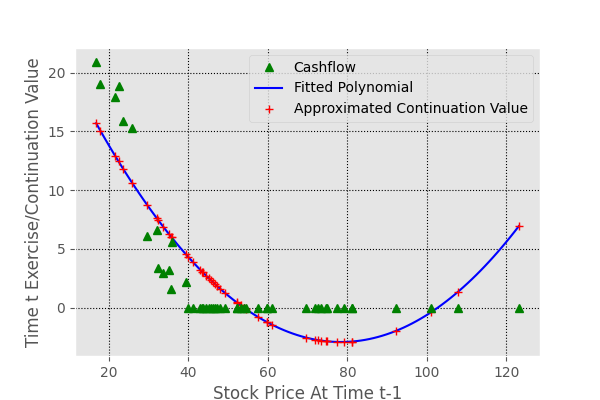
\includegraphics{Figures/LSMFit1.png}
\decoRule
\caption[Polynomial Regression Of Continuation Value]{By zooming in on a specific point of time in backward induction approach, we see how the algorithm regress the continuation value}
\label{fig:LSM1}
\end{figure}

\subsection{American Put}
The optimal stopping problem for an American put 
\begin{equation}\label{optimalStopPut}
\begin{split}
P(0) = \sup_{\tau \in \mathcal{T}(0,\ldots,T)} E^Q[ e^{-r \tau} \cdot \max\{K-S(\tau), 0 \}]
\end{split}
\end{equation}
can be solved with the LSM algortihm. The stock values are modeled via Black-Scholes theory\footnote{Illustration of generated path for the GBM in figure \ref{fig:BM}}, hence the simulated evolution for the stock under the risk neutral valuation is given by:
\begin{equation*}
\begin{split}
S_i(t)=S_i(0) \cdot \exp \bigg( \sum_{j=1}^{d}(\sigma_{i,j} W_j(t) -\frac{1}{2} \sigma_{i,j}^2 t) + rt \bigg) \quad  for \ i=1,\ldots,d
\end{split}
\end{equation*}
The stock paths are simulated from inception up to maturity with N-1 decision dates. The focus in this section is on a univariate contingent claim and for convenience we assume the risk free interest rate and volatility is constant. Like in the binomial model, we work backward from maturity to inception at each exercise dates to decide the optimal stopping time. \\

The dynamic programming principle on optimal policy gives the first optimal stopping time. In our setting we regress the expected payoff by continuation of the contract and compare it to the intrinsic value. The dependent variable in the regression is the expected value of continuation and the independent variables is a set of orthogonal basis functions in $L^2(\sigma(S(t_n)))$ of the simulated paths. Typical choices for basis functions could be weighted Laguerre -, Hermit -, and Jacob polynomials. The weighted Laguerre polynomial is given by
\begin{align*}
e_0(S) &= \exp(-S/2) \\
e_1(S) &= \exp(-S/2) (1-S) \\
e_2(S) &= \exp(-S/2) (1-2S+S^2/2) \\
\vdots \\
e_j(S) &= \exp(-S/2) \dfrac{e^S}{j!} \frac{d^j}{dS^j}(S^j e^{-S}) 
\end{align*} 
This kind of regression is a nonlinear expansion of the linear model. We define regressed conditional expectation by:
$$\Psi(S; \alpha)= \sum_{j=0}^p \alpha_j \cdot e_j(S) $$
where $\alpha$ is the coefficients for the regression, e is the basis function, where the argument is the underlying Markovian process $S$. By using this iterative method, we arrive at the pathwise optimal stopping policy, where in figure \ref{fig:LSM2} the optimal stopping times are shown. The figure illustrates that the option only can be exercised once, hence the gray lines after the triangles.

\begin{figure}[th]
\centering
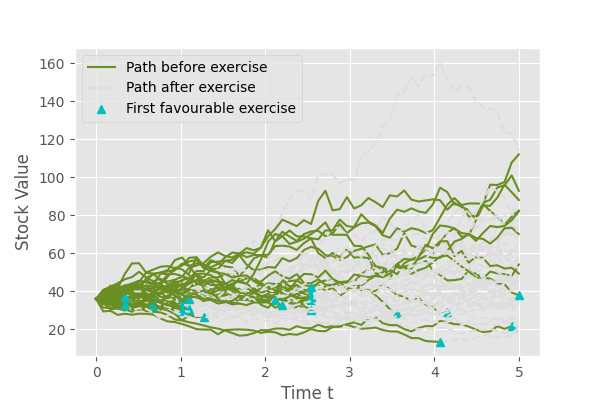
\includegraphics{Figures/LSMFit2.png}
\decoRule
\caption[Optimal Stopping Decision]{The optimal stopping decisions by the Least Square Monte Carlo Method}
\label{fig:LSM2}
\end{figure}

Note (TODO!) that for practical implementation the LSM only consider in the money path, hence equation \eqref{LSMestimator} is changed to:
\begin{equation*}
\alpha^{(m,K)}(t_n)= \argmin_{a\in \mathbb{R}^m} \dfrac{1}{K}\sum_{k=1}^{K^{ITM}} \bigg(G(S^{(k)}(\tau^{k,m,K}_{t_{n+1}}))  -a \cdot e^m(S^{(k)}(t_{n})) \bigg)^2 \quad for \ n=1, \ldots, N-1
\end{equation*}
Where $K^{ITM}$ means we only consider ITM paths.


\subsection{Convergence}
In the rigorous approach in \parencite{analysisLSM} they show convergence results for the optimal value process or the Snell envelope $U$. We will present that $U(0)^{m,K}$ converges almost surely to $U(0)^{m}$ for K goes to infinity, i.e. the approximate value process by simulation and regression on a finite set of functions converge to the approximated value process with truncated orthogonal basis by letting the sample size go to infinity. Furthermore it can be shown that $U(0)^{m}$ converge to $U(0)$ for m goes to infinity. The second result is that the regressed value function converge to the expected continuation value by letting the number of basis function goes to infinity. The latter result is shown using the expected continuation values.
\begin{theorem}\label{LSMConvergence1}
Assume the sequence $(e_{j}(S(t_n)))_{j\geq 1}$ is total in $L^2(\sigma(S(t_n)))$ for $n=1,\ldots,N-1$. Then for $n=0,\ldots,N$ we have
$$\lim_{m\to +\infty} E^Q[G(S(\tau_{t_n}^{[m]})) |\mathcal{F}_{t_n}]=E^Q[G(S(\tau_{t_n})) |\mathcal{F}_{t_n}]$$
in $L^2$
\begin{proof}
The proof is given by induction, where the orthogonal basis is total in $L^2$ is important, because $||P^m_{t_n}(E^Q[G(S(\tau_{t_{n+1}}))|\mathcal{F}_{t_n}])- E^Q[G(S(\tau_{t_{n+1}}))|\mathcal{F}_{t_n}]||_2 \to 0 \quad for \ m \to \infty$.
(more details on p. 6-7 \parencite{analysisLSM})
\end{proof}
\end{theorem}

The former result is also shown in \parencite{analysisLSM}.
\begin{theorem}\label{LSMConvergence2}
Assume the sequence $(e_{j}(S(t_n)))_{j\geq 1}$ is total in $L^2(\sigma(S(t_n)))$ for $n=1,\ldots,N-1$ and if $\sum_{j=1}^{m} \lambda_j e_{j}(S(t_n))=0 \ a.s.$ then $\lambda_j=0$ for $n=1,\ldots,N-1$, $m\geq 1$ and $j=1,\ldots,m$. Furthermore assume that $Q(\alpha_{t_n} \cdot e(S(t_n))=G(S(t_n)))=0$.\\
Then $U^{m,K}(0)$ converges almost surely to $U^{m}(0)$ as K goes to infinity.\\
The proof is out of scope for this thesis, see the article \parencite{analysisLSM} for a proof in details. 
\end{theorem}

The two convergence results shows the convergence for the LSM algorithm, hence the LSM will approximate the optimal value process well for sufficient large sample sets and enough basis functions.


\subsection{Upper Bound}
By the results from \parencite{AndersenLeif2004} they provide a algorithm for computing a lower and upper bound for the American option price, where the lower bound is generated by approximating the continuation value. They show with martingale methods that the interval becomes smaller when the lower bound approaches the true value. The true value will always by higher than the approximation, because the true value is when you exercise optimal at each decision point. Hence to compare approximation method on the continuation value a higher lower bound indicate a better approximation to the true value.

Given the optimal exercise boundary is only an estimate, both the methods underestimate the "true value" of the option.

A simple comparison would be whichever method produced higher price for the option is better.

For this comparison to make sense, you could

    re-use underlying stock simulation across both the methods.
    make sure variance of price produced is reasonably low for both.

The "better" value of the two is still a lower bound and doesn't really throw information on how big the error is.

You could implement dual method to produce upper bound and thus a range for the true option price.
The regression performed in LSM is only for in money path for improving the algorithm, wher



The LSM approach gives a lower bound for the true price of the option given optimal stopping choice:
\theoremstyle{proposition}
\begin{proposition}{}\label{Lower-Bound-LSM}
\textbf{Lower Bound To True Value:} For any finite choice of M, K, and vector $\theta\in \mathbb{R}^{M \times (K-1)}$ representing the coefficients for the M basis functions at each of the K-1 early exercise dates, let $LSM(\omega;M,K)$ denote the discounted cash flow resulting from the following the LSM rule of exercising when the immediate exercise value is positive and greater than or equal to $\hat{F}_{M}(\omega_{l};t_{k})$ as defined by $\theta$. Then the following inequality holds almost surely,
$$V(X)\geq \lim_{N\to \infty} \dfrac{1}{N}\sum_{i=1}^{N} LSM(\omega_i;M,K)$$
(p. 124 \parencite{LSM})
\end{proposition}


\subsection{LSM Extension To Multivariate Contingent Claims}
For pricing of bivariate and multivariate contingent claims, we have to account for correlation between assets. The correlation matrix $\Sigma$ is given by
\begin{equation}
\Sigma = \begin{pmatrix}
\rho_{1,1} & \rho_{1,2} & \cdots & \rho_{1,d} \\
\rho_{2,1} & \rho_{2,2} & \cdots & \rho_{2,d} \\
\vdots & \vdots & \ddots & \vdots \\
\rho_{d,1} & \rho_{d,2} & \cdots & \rho_{d,d} \\
\end{pmatrix} = \Sigma = \begin{pmatrix}
1 & \rho_{1,2} & \cdots & \rho_{1,d} \\
\rho_{2,1} & 1 & \cdots & \rho_{2,d} \\
\vdots & \vdots & \ddots & \vdots \\
\rho_{d,1} & \rho_{d,2} & \cdots & 1 \\
\end{pmatrix}
\end{equation}
The correlation between assets are given by $(\rho_{i,j})_{i\neq j}$ and each asset has correlation 1 with itself. We assume that $(\rho)_{i \neq j} \in (-\frac{1}{d-1},1]$, because then the correlation matrix is a real, symmetric and positive definite, hence Cholesky factorization can be utilized $\Sigma=LL^T$ where $L$ is a lower triangular matrix. From the decomposition it is easy to simulate correlated assets in d-dimensional Black-Scholes model:
\begin{equation}
dS_{i}(t)=S_{i}(t) r dt + S_{i}(t) \sigma_i L_{i,\cdot} d\bm{W}(t) \quad i \in \{1,2,\ldots, d\}
\end{equation}
Where $\bm{W}$ has values in $\mathbb{R}^d$ and $\sigma=(\sigma_1, \sigma_2, \ldots, \sigma_d)$ is vector of volatilities.\\

By simulating the paths according to the Black-Scholes dynamic, it is straightforward to apply the LSM, because it follows the same algorithm just with a different contract function.

\newpage

%----------------------------------------------------------------------------------------
%	SECTION 4
%----------------------------------------------------------------------------------------

\section{Closed Form Solutions For European Exotic Options}\label{ExoticEuro}
Most exotic options require numerical methods, but in some special cases there exist a closed form solution. We will look at some of them in this section, where the purpose is to provide benchmarks for the numerical methods. Furthermore we explore the boundaries of closed form solutions and show applications of martingale theory. Throughout the financial model and assumptions given in section \ref{MultiDimModel} will be assumed. We derive closed form solutions to European call and put options depending on several variables, for simplicity we will focus on pricing options with 2 or 3 underlying stocks. We apply the intuition given in \parencite{Johnson87} and the results given in \parencite{Ouwehand2006}. The exotic contingent claims we will consider are the geometric mean -, maximum - and minimum call option.

\subsection{Geometric Basket Call Option}\label{GeoBasket}
For a geometric basket call option the contract function is given by:
\begin{align*}
\Phi(S(T))=\max\{ (\prod_{i=1}^{n} S_i(T))^{\frac{1}{n}}-K,0 \}
\end{align*}
The key to  derive a closed form solution is the known result that the sum of normal random variables are multivariate normal distributed.
This implies that the product of lognormal random variables are multivariate log-normal distributed. Since: 
\begin{equation*}
\begin{split}
\exp(x+y)&=\exp(x)\cdot \exp(y) \\
& \text{and}\\
 X \sim \mathcal{N}(\mu,\sigma^2) & \Rightarrow Y = \exp(X)\sim LN(\mu, \sigma^2)
\end{split}
\end{equation*}

Remember the assumption in section \ref{MultiDimModel} that the stock price process follows a GBM, hence:
\begin{equation}\label{prodGBM}
\begin{split}
(\prod_{i=1}^{d} S_i(T))^{\frac{1}{d}} = (\prod_{i=1}^{d} S_i(0))^{\frac{1}{d}} \exp\bigg((r-\frac{1}{2d}\sum_{i=1}^{d}\sigma_i^2)T + \frac{1}{d} \sum_{i=1}^{d} \sigma_i W_i(T) \bigg)
\end{split}
\end{equation}
By defining
\begin{align}
\tilde{\sigma} = \frac{1}{d} \sqrt{\sum_{i=1}^{d} \sigma_i^2 + 2 \sum_{i\neq j} \rho_{i,j} \sigma_i \sigma_j}\\
F=(\prod_{i=1}^{d} S_i(0))^{\frac{1}{d}} \exp\bigg((r-\frac{1}{2d}\sum_{i=1}^{d}\sigma_i^2)T + \frac{1}{2} \tilde{\sigma}^2 \cdot T \bigg)\\
\epsilon = \frac{\frac{1}{d} \sum_{i=1}^{d} \sigma_i W_i(T)}{\tilde{\sigma} \sqrt{T}} \sim \mathcal{N}(0,1)
\end{align}
Rewrite equation \eqref{prodGBM} by above definitions
$$(\prod_{i=1}^{d} S_i(T))^{\frac{1}{d}} = F \cdot \exp\bigg( -\frac{1}{2} \tilde{\sigma}^2 \cdot T + \tilde{\sigma} \sqrt{T} \epsilon \bigg)$$
This expression is one dimensional and is the standard GBM solution with zero drift and spot F. This has a known solution with Black-Scholes theory (section \ref{classicBS}) and the geometric mean call option has price
\begin{equation*}
\Pi(t,\mathcal{X})=\exp(-r \cdot (T-t))\bigg(F N(d_1) - K N(d_2) \bigg)
\end{equation*}
where $d_1=\frac{\ln(\frac{F}{K}) + \frac{1}{2} \tilde{\sigma}^2 T}{\tilde{\sigma} \cdot \sqrt{T}}$ and $d_2=d_1-\tilde{\sigma} \sqrt{T}$\\

The fact that the sums of normal random variables is multivariate normal distributed makes the geometric mean option easy to price in the Black-Scholes model, because the high dimensional problems can be treated as 1-dimensional problem like above with the European geometric mean call option.

\subsection{Options On The Maximum Or The Minimum Of Several Assets}
Here we restrict ourselves to consider the case with three underlying stocks like in \parencite{BEG, Ouwehand2006}, but the formula can be generalized to higher dimensions. The contract functions we consider are:
\begin{enumerate}
\item[•] Best of assets or cash: $\Phi(S(T))=\max\{S_1,S_2,\ldots,S_d,K\}$
\item[•] Call on max: $\Phi(S(T))=\max\{\max(S_1,S_2,\ldots,S_d)-K,0\}$
\end{enumerate}
Assume WLOG $d$=4 to avoid cumbersome calculations and notation. The section will heavily use the martingale framework developed in section \ref{MultiDimModel} and stochastic calculus (Appendix \ref{AppendixB}) to value these exotic options. The key is to choose the numéraire to a risky assets instead of the bank account. By results from section \ref{MultiDimModel} the processes are still Q-martingales given the numéraire is strictly positive. Under the assumption of a arbitrage free and complete market it follows from risk neutral valuation formula(RNVF).
$$S_0(t)E^{Q_0}_t[\frac{X}{S_0(T)}]=S_1(t)E^{Q_1}_t[\frac{X}{S_1(T)}]$$
This show that changing the numéraire does not change the price of the above derivative.

\subsubsection{Best Of Assets Or Cash}
The best of assets derivative will provide the foundation for pricing call on maximum or minimum of several assets. The best of assets derivative pay out the price of the most valuable asset. The idea is then to set up 4 cases, where in each case a new asset gives a payout if it is the most valuable out of the four cases. This can be written with a indicator, where the payoff for the $i$'th asset is:
\begin{equation}\label{ithPayoff}
S_i(T) \cdot 1_{\{S_i(T)>S_j(T): i\neq j\}} \quad i=\{1,2,3,4\}
\end{equation}

From equation \eqref{ithPayoff} we see that the i'th assets is only different from zero, when it is the most valuable asset. The best of asset derivative is then a sum of 4 terms (remember d=4), where each term is equation \eqref{ithPayoff} for a specific asset $i$. Hence the best of asset derivative can be consider as a sum of 4 derivatives, where we apply RNVF (proposition \ref{RNVF}) for each of them.\\

Let us first consider i=1 and we set $S_1$ to be the numéraire asset with martingale measure $\mathbb{Q}_1$. Then by RNVF:
\begin{equation}\label{ithDerivative}
\begin{split}
\Pi_1(t, \mathcal{X})&=S_1(t)E_t^{Q_1}[1_{\{S_1(T)>S_2(T), S_1(T)>S_3(T), S_1(T)>S_4(T)\}}]\\
&=S_1(t) Q_1[\ln(\frac{S_2(T)}{S_1(T)})<0, \ln(\frac{S_3(T)}{S_1(T)})<0, \ln(\frac{S_4(T)}{S_1(T)})<0]
\end{split}
\end{equation}
From above discussion the derivative price can be found by cycling through the 4 derivatives and add together the prices of the four derivatives. The fair price for best of assets option $\Pi_{max}(t,\mathcal{X})$ is then given as the sum of the 4 derivatives. The above derivative equation \eqref{ithDerivative} needs to be evaluate, therefore we seek to evaluate the probability under the $Q$-martingale measure. By Ito's lemma (see \ref{Ito}) the discounted process with stock j is
\begin{align}
d(\dfrac{S_i(t)}{S_j(t)})=\frac{S_i(T)}{S_j(T)} \cdot (a_i-a_j)dW^{Q_j}(t) 
\end{align}
where $dW^{Q_j}(t)$ is standard d-dimensional $Q_j$-Wiener process and $a_i$ is the i'th row of the covariance matrix. From the known solution of the GBM we have the distribution.
\begin{align*}
\ln(\frac{S_i(T)}{S_j(T)})\sim \mathcal{N}\bigg(\ln(\frac{S_i(t)}{S_j(t)}) - \frac{1}{2}\sigma_{i/j}^2 \cdot (T-t), \sigma_{i/j}^2 (T-t)\bigg)
\end{align*}
where $\sigma_{i/j}=(a_i-a_j)$ and $\sigma_{i/j}^2=\sigma_i^2+\sigma_j^2-2\rho_{ij}\sigma_i \sigma_j$.\\

Besides using the definition for $d_1$ and $d_2$ in proposition \ref{BS-price-EuroCall} we define:
\begin{align}
d^{i/j}_1 =\frac{1}{\sigma_{i/j}\cdot \sqrt{T-t}} \cdot \bigg( \ln(\frac{S_i(t)}{S_j(t)}) + \frac{1}{2} \sigma_{i/j}^2 \cdot (T-t) \bigg)\\
d^{i/j}_2=d^{i/j}_1-\sigma_{i/j} \sqrt{T-t}
\end{align}
The correlation between $\frac{S_i(T)}{S_k(T)}$ and $\frac{S_j(T)}{S_k(T)}$ is:
\begin{align}
\rho_{ij,k}&:= \dfrac{(a_i-a_k)\cdot(a_j-a_k)}{||a_i-a_k|| \cdot ||a_j-a_k||}\\
&=\frac{\rho_{ij}\sigma_i \sigma_j - \rho_{ik}\sigma_i \sigma_k - \rho_{kj}\sigma_k \sigma_j + \sigma_k^2}{\sqrt{(\sigma_i^2 + \sigma_k^2 - 2\rho_{ik}\sigma_i \sigma_k)\cdot(\sigma_j^2 + \sigma_k^2 - 2\rho_{jk}\sigma_j \sigma_k)}}
\end{align}
Hence:
$$Q_1[\ln(\frac{S_2(T)}{S_1(T)})<0, \ln(\frac{S_3(T)}{S_1(T)})<0, \ln(\frac{S_4(T)}{S_1(T)})<0]=N_3(-d_2^{2/1},-d_2^{3/1},-d_2^{4/1}, \rho_{23,1}, \rho_{24,1}, \rho_{34,1})$$
Cycling through each derivative, we get:
\begin{equation}\label{BestAsset}
\begin{split}
\Pi_{max}(t,\mathcal{X})&=S_1(t) N_3(-d_2^{2/1},-d_2^{3/1},-d_2^{4/1}, \rho_{23,1}, \rho_{24,1}, \rho_{34,1}) \\
&+S_2(t) N_3(-d_2^{1/2},-d_2^{3/2},-d_2^{4/2}, \rho_{13,2}, \rho_{14,2}, \rho_{34,2})\\
&+S_3(t) N_3(-d_2^{1/3},-d_2^{2/3},-d_2^{4/3}, \rho_{12,3}, \rho_{14,3}, \rho_{24,3}) \\
&+S_4(t) N_3(-d_2^{1/4},-d_2^{2/4},-d_2^{3/4}, \rho_{12,4}, \rho_{13,4}, \rho_{23,4})
\end{split}
\end{equation}
We can extend the above result to best of assets and cash by letting $S_4(t)=K\exp(-r(T-t))$, where K do not have any volatility and also independent of the other assets, hence \eqref{BestAsset} becomes:
\begin{equation}\label{BestAssetOrCash}
\begin{split}
\Pi_{max}(t,\mathcal{X})&=S_1(t) N_3(-d_2^{2/1},-d_2^{3/1},d_1^{1}, \rho_{23,1}, \rho_{24,1}, \rho_{34,1}) \\
&+S_2(t) N_3(-d_2^{1/2},-d_2^{3/2},d_1^{2}, \rho_{13,2}, \rho_{14,2}, \rho_{34,2})\\
&+S_3(t) N_3(-d_2^{1/3},-d_2^{2/3},d_1^{3}, \rho_{12,3}, \rho_{14,3}, \rho_{24,3}) \\
&+K\cdot \exp(-r(T-t)) N_3(-d_2^1,-d_2^2,-d_2^3, \rho_{12}, \rho_{13}, \rho_{23})
\end{split}
\end{equation}

\subsubsection{Call On Max And Call On Min}
From the price of the best of asset or cash option equation \eqref{BestAssetOrCash} the call max option price can be derived. Note that
$$\max\{\max\{ S_1,S_2,S_3 \} - K, 0\}=\max\{\max\{ S_1,S_2,S_3 \}, K\} - K = \max\{ S_1,S_2,S_3,K \} - K$$
The call on max option is then a best of asset or cash option subtracted the strike. Realizing that fact it is easy to price the call on max:
\begin{equation}\label{callMax}
\begin{split}
\Pi_{cmax}(t,\mathcal{X})&=S_1(t) N_3(-d_2^{2/1},-d_2^{3/1},d_1^{1}, \rho_{23,1}, \rho_{24,1}, \rho_{34,1}) \\
&+S_2(t) N_3(-d_2^{1/2},-d_2^{3/2},d_1^{2}, \rho_{13,2}, \rho_{14,2}, \rho_{34,2})\\
&+S_3(t) N_3(-d_2^{1/3},-d_2^{2/3},d_1^{3}, \rho_{12,3}, \rho_{14,3}, \rho_{24,3}) \\
&-K \exp(-r(T-t)) \cdot\bigg(1 - N_3(-d_2^1,-d_2^2,-d_2^3, \rho_{12}, \rho_{13}, \rho_{23})\bigg)
\end{split}
\end{equation}

To derive put max we can utilize a put-call-parity (page 6 \parencite{Ouwehand2006}), but it takes a different form than the one presented in \ref{Chapter2} (proposition \ref{put-call-parity}). The relationship for the exotic European call options:
\begin{equation}\label{putMin}
V_c(K)+K\exp(-r\cdot (T-t)) = V_p(K)+V_c(0)
\end{equation}
Where $V_c(K)$ is the value of the exotic European call option and $V_c(0)$ is the best of assets call option.\\

The exotic European options serve as benchmark for the multivariate lattice approach, because if the lattice approach is close to the European benchmark then it is reasonable to expect a close estimate to the American option. The above section is also a presentation of the martingale approach versatility. 



